%%%%%%%%%%%%%%%%%%%%%%%%%%%%%%%%%%%%%%%%%%%%%%%%%%%%%%%%%%%%%%%%%%%%%%
% How to use writeLaTeX:
%
% You edit the source code here on the left, and the preview on the
% right shows you the result within a few seconds.
%
% Bookmark this page and share the URL with your co-authors. They can
% edit at the same time!
%
% You can upload figures, bibliographies, custom classes and
% styles using the files menu.
%
% If you're new to LaTeX, the wikibook is a great place to start:
% http://en.wikibooks.org/wiki/LaTeX
%
%%%%%%%%%%%%%%%%%%%%%%%%%%%%%%%%%%%%%%%%%%%%%%%%%%%%%%%%%%%%%%%%%%%%%%
\documentclass{tufte-handout}

%\geometry{showframe}% for debugging purposes -- displays the margins

\usepackage{amsmath}

% Set up the images/graphics package
\usepackage{graphicx}
\setkeys{Gin}{width=\linewidth,totalheight=\textheight,keepaspectratio}
\graphicspath{{graphics/}}

\title{Hands-On Session: Intro to ietestform}
\author{DIME Analytics \\ dimeanalytics@worldbank.org}
\date{11 June 2019}  % if the \date{} command is left out, the current date will be used

% The following package makes prettier tables.  We're all about the bling!
\usepackage{booktabs}

% The units package provides nice, non-stacked fractions and better spacing
% for units.
\usepackage{units}

% The fancyvrb package lets us customize the formatting of verbatim
% environments.  We use a slightly smaller font.
\usepackage{upquote}
\usepackage{fancyvrb}
\fvset{fontsize=\normalsize}
\renewcommand{\FancyVerbFormatLine}{\color{violet}}
\DefineShortVerb{\|}

% Small sections of multiple columns
\usepackage{multicol}

% Provides paragraphs of dummy text
\usepackage{lipsum}

% These commands are used to pretty-print LaTeX commands
\newcommand{\doccmd}[1]{\texttt{\textbackslash#1}}% command name -- adds backslash automatically
\newcommand{\docopt}[1]{\ensuremath{\langle}\textrm{\textit{#1}}\ensuremath{\rangle}}% optional command argument
\newcommand{\docarg}[1]{\textrm{\textit{#1}}}% (required) command argument
\newenvironment{docspec}{\begin{quote}\noindent}{\end{quote}}% command specification environment
\newcommand{\docenv}[1]{\textsf{#1}}% environment name
\newcommand{\docpkg}[1]{\texttt{#1}}% package name
\newcommand{\doccls}[1]{\texttt{#1}}% document class name
\newcommand{\docclsopt}[1]{\texttt{#1}}% document class option name

\begin{document}

\maketitle% this prints the handout title, author, and date

\begin{marginfigure}%
  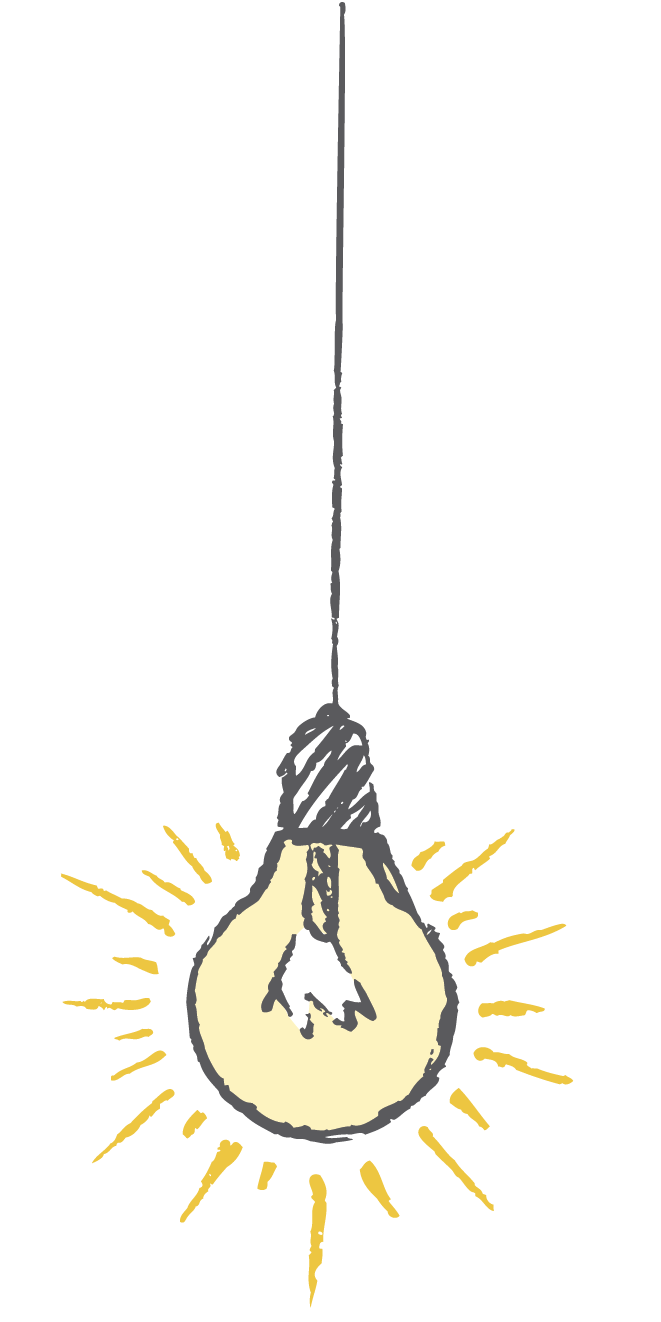
\includegraphics[width=\linewidth]{img/light.png}
\end{marginfigure}

\begin{abstract}
This Exercise will introduce new users to the features of the command \textbf{ietestform} that is developed by DIME Analytics. \textbf{ietestform} bring together years of experience at DIME in how to code high quality SurveyCTO questionnaires.


\bigskip\noindent \textbf{Exercise Objectives}:
\begin{enumerate}
  \item Learn how to run the command
  \item Learn what the most common tests are testing for and why
  \item Learn how to use the documentation 
\end{enumerate}
\end{abstract}

%\printclassoptions
\section{Intro and context for the exercise}

	Coding a complex questionnaire is difficult, especially since it next to impossible to keep a good overview of your Excel form template once it reached several hundreds of rows of code which is the norm rather than the exception.
	
	While it ends up being very challenging for a human eye to catch a typo in a single out of hundreds of row, that is pose no challenge to a computer once we have developed a way to express in code what is very likely a typo. One example is if we have 10 multiple choice list items, where 9 of them have the list name \textit{village} and one have the list name \textit{vilage}, and the list \textit{vilage} is not used. We can express a test like that in code, and that one example of the many test that \verb|ietestform| is developed to do on your SurveyCTO forms.
	
	Other examples are test that no fields of type \textit{note} are required, test that no two multiple choice codes has the same label, test that non standard characters are used in field names that will later cause problem when loading it in Stata. Sometimes some of these things are intentional, so all the cases that \verb|ietestform| flag are not always errors, but a human should pay extra attention to each case flagged to see whether it is an error or not.

%\printclassoptions
\section{Part 1: Run ietestform}

	We have prepared a do-file\sidenote{see the file handson\_iestestform.do provided in the excercise material or in the code example below} for you that make sure you have |ietoolkit| and |iefielkit| installed and that you are using the most recent version of |iefieldkit|. It also uses |ieboilstart| to harmonize version and memory settings, and lastly sets up a global path file to the folder we will work in before it runs the command.
	
	After you have filled in your user name\sidenote{In \verb|"`c(username)'" == ""| replace the \verb|""| with your computers username} and your file path\sidenote{In \verb|global folder ""| replace the \verb|""| with your file path} to the folder you want to use for this exercise, you can run this do-file and then the report will be created in the folder you specified in the folder global. Once you have been able to generate the report, move to next step.


	\begin{minipage}{1.5\textwidth}
	\vspace{.5cm}
	\VerbatimInput[frame=lines, % line above and below code section
	 			   numbers=left, %Line number
	 			   label=handson\_ietestform.do, %name of code section
	 			   samepage=true, %Do not allow the code to be broken across pages
	 			   baselinestretch=0.75 %Use line space more similat to line space in code editors
	 			  ]{./handson_ietestform.do}
 	\end{minipage}


%\printclassoptions
\section{Part 2: Read the output}

	If the code ran successfully a report will have been created in the folder location you specified in the do-file. In the output window in Stata there will also be a hyper link to the file. Open the report either by clicking the link of clicking the file in the folder. 
	
	At the top of the file there are a section of meta-information on the how the report was generated. The first line indicates the username of the computer used to generate this report, when it was done and that it was ietestform that generated the report. This will be useful when a member of the research team in the future is looking at this report.
	
	Then there are two links to documentation, and lastly there is meta data about the form. Apart from the \textit{Form File} all these values are taken from the settings tab in the Excel file form definition. The \textit{Form File} value is the name of the file specified in the do-file when running |ietestform|.

	\begin{minipage}{1.5\textwidth}
		\vspace{.5cm}
	 	\begin{Verbatim}[frame=lines,
						numbers=left,
						label=ietestform-header,
						samepage=true,
						baselinestretch=0.75]

This report was created by user kbrkb on 15May2019 using the Stata command ietestform

Use either of these links to read more about this command:
	https://github.com/worldbank/iefieldkit
	https://dimewiki.worldbank.org/wiki/Ietestform

	Form ID      GHANA_instrument
	Form Title   GHANA_instrument
	Form Version 1905141904
	Form File    ietestform-handson-session-cto-form.xls
		\end{Verbatim}
		\vspace{.5cm}
 	\end{minipage}
 
	\noindent The rest of the report is organized in small section where each section corresponds to the result of a test. Tests that did not generate any results are not shown, so there are no "empty" sections. Each section follow the same format. First a title with the name of the test, then a sort description of which variables in which sheet the test found this case reported on, and then there is a section listing the cases found. Often this is a table like in the example below, but that is not aways applicable. The variable row does not exist in the Excel file, it is just a reference to the row in the excel sheet.
	
	Finally there is a link to the wiki page for this command where both the test and the underlaying best practice is explained in more detail. Whenever you are not sure why something is in the report of |ietestform| always start by reading the information on the linked wiki page. Not all cases found by |ietestform| are necessarily errors, but they should always be followed up on.
 	
	\begin{minipage}{1.5\textwidth}
	 	\vspace{.5cm}
	 	\begin{Verbatim}[frame=lines,
	 					numbers=left,
	 					label=ietestform-test-section-example,
	 					samepage=true,
	 					baselinestretch=0.75]
	 	
----------------------------------------------------------------------
TEST: MISSING LIST LABELS
----------------------------------------------------------------------
There non-missing values in the [name] column of the choice sheet 
without a label in the [label] colum:
 
  row list_name name label        labelSpanish 
  12  exam      2    BP Apparatus 
  18  exam      7                 Pulse_2
 
 Read more about this test and why this is an error or does not follow 
 the best practices we recommend here:
 https://dimewiki.worldbank.org/wiki/Ietestform#Missing_Labels_or_Value.2FName_in_Choice_Lists

		\end{Verbatim}
		\vspace{.3cm}
	\end{minipage}

%\printclassoptions
\section{Part 3: Common tests}

	For this exercise we have prepared a questionnaire form where we intentionally have included a lot of different type of things that |ietestform| will report on. Part 4 will discuss how to use the documentation to understand more uncommon cases once you encounter them, but this section will focus on more common cases.
	
	SurveyCTO's server perform a test when you are uploading a questionnaire. However, in order for them to allow innovative ways of coding they cannot make that test too strict. And that test only reports direct syntax errors that the software does not know how to run. There is no middle ground for warnings for risky practices, or warnings for practices that sometimes are correct but often are unintentional and can cause major complications while in the field. That is where this command comes in. 
	
	|ietestofrm| is not a substitute to the test on SurveyCTO's server, it is a compliment. The questionnaire form used in this exercise uploads without errors to SurveyCTO's server, but as you will see, it is full of practices that can lead to complications.

\subsection{MISSING LIST LABELS}
	Find the \textit{TEST: MISSING LIST LABELS} in the report you generated and find these cases in the Excel questionnaire form. Remember that the column row list which Excel row this case can be found at. Answer the following questions, and use the documentation linked to in the report for this test when you do not know the answer:
	
	\begin{enumerate}
		\item What could go wrong if this case is not addressed?
		\item Is there a case when this will not be found during testing? 
		\item For a language like Spanish - which is used in this example - it is likely that the person coding the questionnaire will speak the language and test in all languages. Will that be the case for all local languages in the type of countries where we operate?
	\end{enumerate}

\subsection{REQUIRED NOTE TYPE FIELD}
	Find the \textit{TEST: REQUIRED NOTE TYPE FIELD} in the report you generated and find these cases in the Excel questionnaire form.
	
	\begin{enumerate}
		\item What could go wrong if this case is not addressed?
		\item Can you come up with one case when it is correct to intentionally have a required field of type note?
	\end{enumerate}

\subsection{UNUSED CHOICE LISTS}
	Find the \textit{TEST: UNUSED CHOICE LISTS} in the report you generated and find these cases in the Excel questionnaire form.
	
	\begin{enumerate}
		\item What is a case found by this test usually a sign of? 
	\end{enumerate}
	
	\noindent It is not always wrong to have a form with some unused choice list. But as in all coding, you are much less likely to make mistake if you keep your code cleaned up.

\subsection{DUPLICATED LABEL WITHIN LIST}
	Find the \textit{TEST: DUPLICATED LABEL WITHIN LIST} in the report you generated and find these cases in the Excel questionnaire form.
	
	\begin{enumerate}
		\item What could go wrong if this case is not addressed?  
	\end{enumerate}

\subsection{SPACES BEFORE OR AFTER STRING (choice sheet)}
	Find the \textit{TEST: SPACES BEFORE OR AFTER STRING (choice sheet)} in the report you generated and find these cases in the Excel questionnaire form.
	
	\begin{enumerate}
		\item What could go wrong if this case is not addressed?   
		\item Will this be an error in all use cases? 
	\end{enumerate}

	SurveyCTO's does not assume that the data will be analyzed in any specific software, so their test does not test for anything that will be an issue first when the data is imported to - for example - Stata. This is an example where |ietestform| test the SurveyCTO code based on the assumption that it will eventually be imported into Stata.

%\printclassoptions
\section{Part 4: Use the documentation}
If you have extra time, go over the rest of the tests in the report, and use the documentation to figure out what the test is testing for and why it is important that the person programming the questionnaire pays extra attention to the case reported on. 

\end{document}
